\documentclass{article}
\usepackage[utf8]{inputenc}
\usepackage{fullpage}
\usepackage{color}
\usepackage{graphicx}
\usepackage{tikz}
\usepackage{pgfplots}
\usepackage{amsmath,amssymb}
\usepackage{bm}
\usepackage{url}

\usepackage{siunitx}
\sisetup{
    detect-all = true,
    input-decimal-markers = {.},
    input-ignore = {,},
    inter-unit-product = \ensuremath{{}\cdot{}},
    multi-part-units = repeat,
    number-unit-product = \text{~},
    per-mode = fraction,
    separate-uncertainty = true,
}

\usepackage[pagebackref,colorlinks,linkcolor=blue,citecolor=blue,urlcolor=blue]{hyperref}

\title{University of Maryland Line Burner Setup}
\author{James P. White}
\date{\today}

\begin{document}

\maketitle

\section{Introduction}

The UMD Line Burner experimental facility provides for the study of a low-strain, buoyancy-driven, fully-turbulent diffusion flame in a canonical line-fire configuration. This facility provides well-controlled inlet and boundary conditions, while introducing the complicating effects of buoyancy and turbulence characteristic of large-scale accidental fires. A variety of non-intrusive diagnostics are employed to measure local and integral flame characteristics. The facility comprises a slot burner centrally located within a surrounding, uniform co-flowing oxidizer. Controlled suppression of the flame is achieved via the introduction of either excess nitrogen gas or a fine water mist into the oxidizer stream. A detailed description of this facility has been presented by White et al.~\cite{White:2015}.

\section{Experimental Description}

A plan view illustration of the burner and oxidizer assembly is presented in Fig.~\ref{fig:umd_line_burner_plan_view}.  The burner features a sand-filled, stainless-steel fuel port, measuring 5 cm wide by 50 cm long, with 1.5 mm thick side walls. Methane gas (99.5 \% purity) or propane gas (99.5 \% purity) are the primary burner fuels. A methane flow rate of 1.00 $\pm$0.02 g/s (nominal 5.4 cm/s) or a propane flow rate of 1.08 $\pm$0.02 g/s (nominal 2.1 cm/s) is utilized, measured using a mass flow controller. Assuming complete combustion, the total heat-release rate is roughly 50 kW for either fuel.

The burner is centrally located at the mouth of a surrounding oxidizer port, measuring 50 cm wide by 75 cm long, with 10 cm thick side walls. Flow conditioning elements ensure that the oxidizer is well-mixed and exits the oxidizer port with a uniform, flat velocity profile. The co-flowing oxidizer is provided at a fixed flow rate of 75$\pm$5 g/s (total, including variable suppressant flow, nominal 22 cm/s), measured using a calibrated pitot-static probe.

Sitting on top of the oxidizer port and surrounding the fuel port is a thin, 5 mm tall, 5 cm wide annulus of ceramic fiberboard, positioned so the top of the board is 10 mm below the lip of the fuel port (and 5 mm above the oxidizer port). This board serves as a flow blockage to reduce the oxidizer velocity near the flame base, forcing the onset of buoyancy-generated turbulence upstream toward the fuel port and reducing the tendency to form laminar structures at the base of the flame.

For nitrogen-dilution suppression experiments, the flame is suppressed via the introduction of a variable flow of gaseous nitrogen into the oxidizer. Suppression potential is characterized by the oxygen mole-fraction in the oxidizer, $X_{O2}$. Quantity $X_{O2}$ is measured using a paramagnetic oxygen analyzer via a probe located in the oxidizer port. The analyzer provides a measurement accuracy of $\pm$0.125 mol \% O2 and a response time of 5 s. An additional transport delay averaging around 20 s, is compensated to provide synchronous data collection with other measurements.

For water-mist suppression experiments, the flame is suppressed via the introduction of a fine water mist into the oxidizer.

Visible flame height is measured using a video camera, defined based on the 50 \% intermittent flame height \cite{White:2015}. These image-based measurements rely on visible flame emissions, including the incandescence of soot particles, and do not strictly locate the stoichiometric flame sheet. The uncertainty in each flame height measurement is less than $\pm$1.5 cm.

Infrared radiative emissions are measured using a water-cooled Schmidt-Boelter heat-flux transducer. The sensor is positioned 100 cm radially outward from the burner centroid, 18 cm above the fuel port, facing perpendicular to the long axis of the burner. This device has a hemispherical absorptance of 0.94 for a spectral range between 0.6-15.0 $\mu$m, a maximum viewing angle of 90\si{\degree}, and a response time of 0.25 s. Measurement accuracy is $\pm$3 \%. The convective portion of the measured heat flux is neglected and sans-flame measurements are applied to correct for background irradiation.

Heat flux data are converted to radiative loss fraction, $\chi_r$, using a weighted multipoint radiation source model, whereby the measured heat flux is assumed to be received from an array of isotropic point sources uniformly distributed over a two-dimensional plane oriented across the visible flame surface [1]. The uncertainty in each $\chi_r$ measurement is less than $\pm$4.5 \%.

Mean and rms temperature data are recorded using an array of R-Type thermocouple probes positioned at selected locations along the centerline of the flame. These probes are constructed using 50 um diameter wires with exposed, bead-welded junctions. Combustion products are collected in an exhaust evacuation system, wherein a gas sampling system provides measurement of the molar concentrations of oxygen ($\pm$0.25 mol \% O2), carbon dioxide ($\pm$1000 ppm CO2), carbon monoxide ($\pm$100 ppm CO), water vapor ($\pm$3 \% RH), and total hydrocarbons ($\pm$10 ppm THC) in the exhaust stream. From these measurements, integral heat release rate and combustion efficiency measurements are derived using species-based calorimetry techniques.

\begin{figure}
\centering
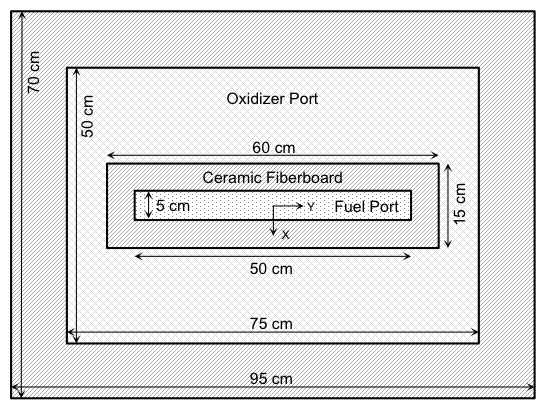
\includegraphics[width=.8\textwidth]{umd_line_burner_plan_view}
\caption{Plan view of burner and oxidizer assembly.}
\label{fig:umd_line_burner_plan_view}
\end{figure}

\section{Simulation Targets}

Available experimental data include:

\begin{itemize}
	\item XO2 at extinction, tabulated
	\begin{itemize}
		\item methane
		\item propane
	\end{itemize}
	\item Flame height vs. XO2
	\begin{itemize}
		\item methane
		\item propane
	\end{itemize}
	\item Heat flux vs. XO2
	\begin{itemize}
		\item methane
		\item propane
	\end{itemize}
	\item Mean thermocouple temperature profiles
	\begin{itemize}
		\item methane, XO2=0.18, $z = 0.125$ m
		\item methane, XO2=0.18, $z = 0.250$ m
	\end{itemize}
\end{itemize}

Pending/planned experimental data include:

\begin{itemize}
	\item HRR / combustion efficiency vs. XO2
	\begin{itemize}
		\item methane
		\item propane
	\end{itemize}
	\item HRR / combustion efficiency vs. spray density
	\begin{itemize}
		\item methane
		\item propane
	\end{itemize}
	\item Mean thermocouple profile/centerline data
	\begin{itemize}
		\item methane, XO2 = 0.21
		\item propane, XO2 = 0.21
	\end{itemize}
	\item RMS thermocouple profile/centerline data
	\begin{itemize}
		\item methane, XO2 = 0.21
		\item propane, XO2 = 0.21
	\end{itemize}
\end{itemize}


\bibliographystyle{plain}
\bibliography{../../../../Utilities/macfp_refs}

\end{document}
